\section{Globales FEM}

FEM-Analysen zur kontrolle der Handrechnungen.\\
Verformungen\\
Überprüfen ob der Boden geklebt werden kann.\\

Was wird rausgelesen:\\
Lagerreaktionen: Deichsel, Links, Rechts\\
Träger A und B Reaktionen:\\
Chassis: Max. Biegemoment.\\
Chassis: Max. Normalkräfte\\
Dach: Max. Normalkräfte\\
Boden: Max. Kraftreaktion\\


\begin{table}[h!]
\centering
\begin{tabular}{lcccccc}
Grösse	&	Einheit	&	x	&	y	&	z	&	Total	&	Berechnet	\\	\hline
\textbf{Lagerreaktionen}	&		&		&		&		&		&		\\	\thickhline
Deichsel	&		&	0	&	3091	&	0	&	3091	&	-1028	\\
Chassis Links	&	N	&	0	&	33997	&	6476	&	34608	&	37300	\\
Chassis Rechts	&		&	0	&	33997	&	-6476	&	34608	&	37300	\\	\hline	\\
\textbf{Träger A und B}	&		&		&		&		&		&		\\	\thickhline
Normalkräfte A	&	N	&	-604	&	12416	&	-215	&	12433	&		\\
Biegemoment A	&	kNmm	&	-4420	&	-176	&	327	&	4436	&		\\
Normalkräfte B	&	N	&	2381	&	15152	&	679	&	15353	&		\\
Biegemoment B	&	kNmm	&	-5386	&	823	&	-333	&	5459	&		\\	\hline	\\
\textbf{Chassis}	&		&		&		&		&		&		\\	\thickhline
Normalkräfte	&	N	&		&		&		&	-48670	&	-44518	\\
Biegemoment	&	kNmm	&		&		&		&	16360	&		\\	\hline	\\
\textbf{Dach}	&		&		&		&		&		&		\\	\thickhline
Normalkräfte	&	N	&		&		&		&	-10469	&	14840	\\
Biegemoment	&	kNmm	&		&		&		&	314	&		\\	\hline	\\
\textbf{Boden}	&		&		&		&		&		&		\\	\thickhline
Normalkräfte	&	N	&		&		&		&	745	&		\\
Schubkräfte	&	N	&		&		&		&	9286	&		\\	\hline
\end{tabular}
\caption{Vorlagetabelle für Resultate aus FEM}% Add 'table' caption
\label{Resultate Vorlage}
\end{table}











\subsection{Idealisierung und Modell}
Schalen und Balken\\
Sandwichkonstuktionen\\
Masse der verwendeten Bauteile, rest mit Pointmass\\

Nodemerge,\\
MPCxxx General joint für Klebeverbindungen via Object generation

\begin{figure}[h]
\centering
\begin{minipage}{.5\textwidth}
  \centering
  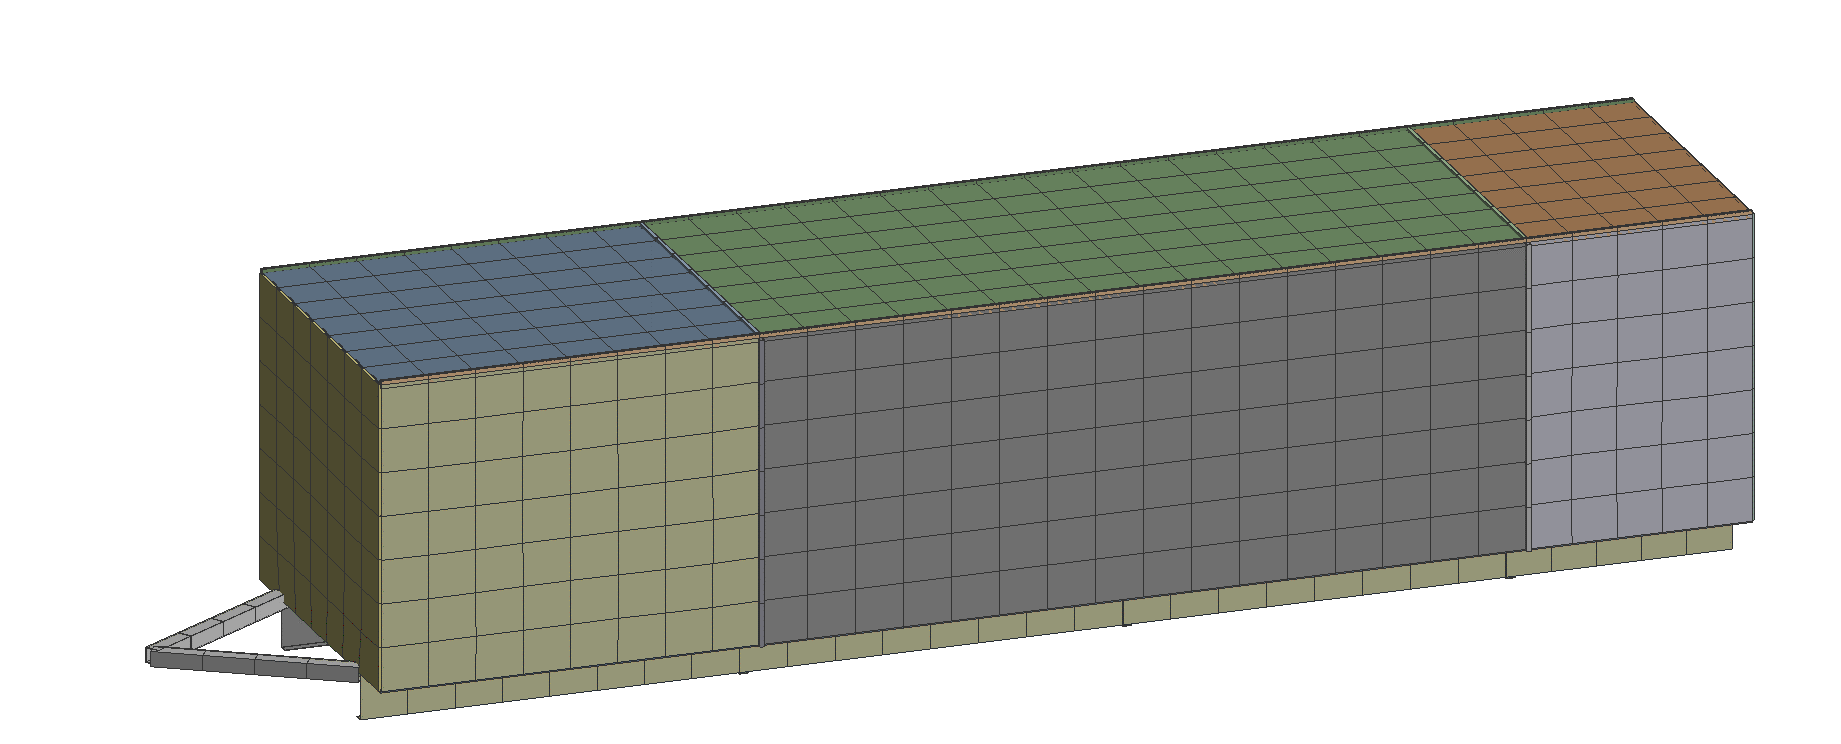
\includegraphics[width=.98\linewidth]{04_figures/FEM Mesh1.png}
  \caption{Darstellung der Balken und Schalenkörper im FEM-Modell}
  \label{FEM Mesh1}
\end{minipage}%
\begin{minipage}{.5\textwidth}
  \centering
  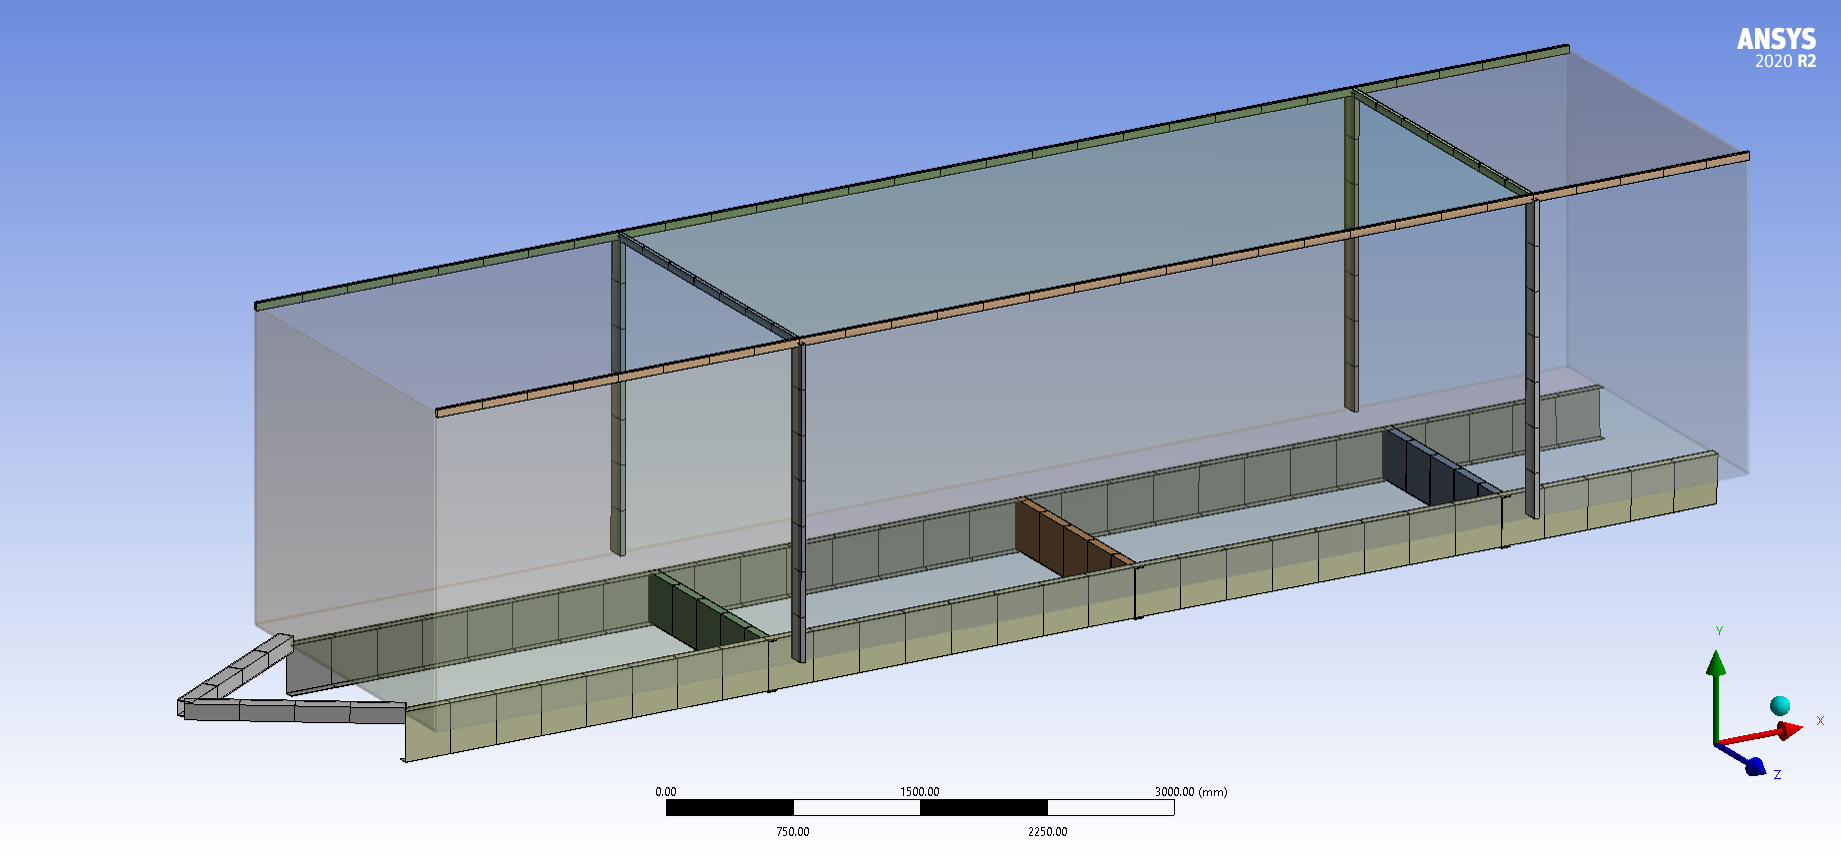
\includegraphics[width=.98\linewidth]{04_figures/FEM Mesh3.png}
  \caption{Darstellung aller Balken im FEM-Modell}
  \label{FEM Mesh3}
\end{minipage}
\end{figure}



\subsubsection*{Vertikale Beschleunigung}


\subsubsection*{Laterale Beschleunigung}


\subsubsection*{Longitudinale Beschleunigung}


\subsubsection*{Rotatorische Beschleunigung}









\newpage
